\chapter{Aufbereitung der Eingabedaten}
Zum Trainieren des Netzes stehen die Windows Schriftarten zur Verfügung. Der Test des Netzwerkes erfolgt im Anschluss mit ungesehenen Schriftarten sowie Handschriftproben der Studenten der Fachhochschule Wedel.

Das Datenmaterial zum Trainieren und Testen wird in \emph{Patternfiles} zur Verfügung gestellt. In diesen Dateien sind die einzelnen Buchstabenformen in einer \emph{14x14} Binärbild-Matrix abgespeichert. Für die Klassifikation wird ein Ausgabevektor mit 26 Dimensionen bereitgestellt. Die Datensätze sind bereits für ein optimales Lernverhalten normiert worden. Hierfür besteht der Wertebereich für das Eingabemuster aus \emph{[-0.5; 0.5]} \imgref{binary_a} und der des Ausgabemusters auf \emph{[0.2; 0.8]} \imgref{binary_alph}.

\begin{figure}[h!]
	\begin{center}
	\fbox{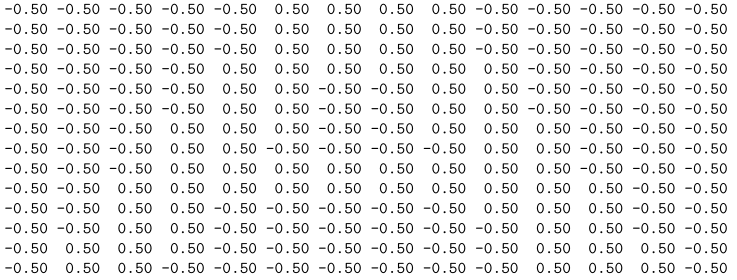
\includegraphics[width=0.9\textwidth]{pictures/binary_a.png}}
	\caption{Eingabemuster mit dem Buchstaben A}
	\label{binary_a}
	\end{center}
\end{figure}

\begin{figure}[h!]
	\begin{center}
	\fbox{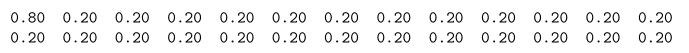
\includegraphics[width=0.8\textwidth]{pictures/binary_alph.png}}
	\caption{Ausgabemuster für den Buchstaben A}
	\label{binary_alph}
	\end{center}
\end{figure}

Die Patternfiles sind nach einem festen Schema \tabref{pattern} aufgebaut welches ein Parsen, in die vom neuronalen Netz benötigte Struktur, ermöglicht.

\begin{table}[h!]
	\centering	
\begin{tabular}{c|c|c}

\textbf{Datensätze} & \textbf{Zeile} & \textbf{Inhalt} \\ 
\hline 
14 & 1 & Zeilen des Eingabemusters \\ 
\hline 
14 & 2 & Spalten des Eingabemusters \\ 
\hline 
1 & 3 & Zeilen des Ausgabemusters \\ 
\hline 
26 & 4 & Spalten des Ausgabemusters \\ 

\end{tabular} 
	\caption{Struktur der Patternfiles}
	\label{pattern}
\end{table}

Über eine einfache Funktion wird das Einlesen der Patternfiles in die für das neuronale Netz benötigte Struktur vorgenommen \lstref{parse}. 
\begin{lstlisting}[caption={Parsen der Patternfiles},label={parse}]
def parseTrainingData(filename):
    ...
    while sampleCount*(inputLines+1)+(inputLines+1) < len(fileArray):
        singleSample = []
        index = 0
        for i in range(4+sampleCount*(inputLines+1), 
                       3+(sampleCount+1)*(inputLines+1)):
            tmp = filter(bool, re.split(" +", fileArray[i].rstrip()))
            singleSample.append(string2floatArray(tmp))
            index = i
        singleOutput = filter(bool, re.split(" +", fileArray[index+1].rstrip()))
        samples.append(tuple([numpy.array(singleSample), singleOutput]))
        sampleCount += 1
        
    return samples
\end{lstlisting}